\documentclass[12pt]{article}

\setlength{\parindent}{0pt}
\setlength{\parskip}{2mm}

\usepackage{geometry}
 \geometry{
 letterpaper, left=20mm, right=20mm,  top=20mm,
 }
\usepackage{graphicx}
\graphicspath{ {graphics/} }
\usepackage{amssymb}
\usepackage{hyperref}
\usepackage{wrapfig}
\usepackage[margin=1.2cm]{caption}
\usepackage{intcalc}
\usepackage{xcolor}
\usepackage{listings}
\lstset{
%	basicstyle=\ttfamily,
	basicstyle=\footnotesize,
  showstringspaces=false,
  commentstyle=\color{red}
}

%%%%%%%%%%%%%%%%%%% TIKZ CUSTOM SHAPES AND SETTINGS
\usepackage{tikz}
\usetikzlibrary{shapes.geometric}
\usetikzlibrary{arrows}
\usetikzlibrary{positioning}
\tikzstyle{hydrophone} = [draw, circle, radius=5mm]
%%%%%%%%%%%%%%%%%%%%%%%%%%%%%%%%%%%%%%%%%%%%%%%%%%%%%%%%%%%%%%%%%%%%%%%%%%%%%%%


%%%%%%%%%%%%%%%%%%%%%%%%%%%%%%%%%%%%%%%%%%%%%%%%%%%%%%%%%%%%%%%%%%%%%%%%%%%%%%%
\begin{document}

%%%%%%%%%%%%%%%%%%%%%%%%%%%%%%%%%%%%%%%%%%%%%%%%%%%%%%%%%%%%%%%%%%%%%%%%%%%%%%%
\begin{titlepage}

\vspace*{5cm}

\begin{huge}
Setup and User Guide
\end{huge}

\begin{large}
Crab Tracker

\vspace*{1cm}

\textbf{Noah Strong}

\vspace*{1cm}
\end{large}

\textit{Revision 1.0-WIP}\\
\today

\vfill
\hfill 
\includegraphics[scale=1]{ct-logo.png}

\end{titlepage}
%%%%%%%%%%%%%%%%%%%%%%%%%%%%%%%%%%%%%%%%%%%%%%%%%%%%%%%%%%%%%%%%%%%%%%%%%%%%%%%
\tableofcontents{}

\newpage

%%%%%%%%%%%%%%%%%%%%%%%%%%%%%%%%%%%%%%%%%%%%%%%%%%%%%%%%%%%%%%%%%%%%%%%%%%%%%%%
\section{Introduction}

The Crab Tracker project was designed as a cost-effective means of remotely
tracking crabs through acoustic signals.
Small piezoelectric transmitters can be waterproofed and attached to crabs,
and their intermittent signals can then be received by a set of four
piezoelectric receivers configured in a square array.

This document will detail the setup and configuration of various elements
of the product as they were originally intended to be used.
As of the time of this writing, some of the hardware elements of this project
are still in development and therefore details about them will not be discussed
in this document.

%%%%%%%%%%%%%%%%%%%%%%%%%%%%%%%%%%%%%%%%%%%%%%%%%%%%%%%%%%%%%%%%%%%%%%%%%%%%%%%
\section{Hardware Setup}

\subsection{Required Hardware Components}

The project was initially built with, and officially supports, the following
devices:
\begin{itemize}
\item \href{https://www.raspberrypi.org/products/raspberry-pi-3-model-b/}
	{Raspberry Pi 3B}
\item \href{https://www.raspberrypi.org/products/raspberry-pi-touch-display/}
	{Raspberry Pi 7" Touch Screen}
\item \href{https://store.arduino.cc/usa/arduino-nano}{Arduino Nano}
\end{itemize}

Additionally, there are transmitters and receivers that were custom designed
for this product.
Specific details about these components are still subject to change as of the
writing of this document, and they will be detailed elsewhere as they are
formalized.
In order to use the Crab Tracker product, it is necessary to fabricate
receiver and transmitter microcontrollers per the specifications detailed
in those documents.
Some of the components must be coated entirely in epoxy for waterproofing.

\subsection{Hydrophone Array}

The Crab Tracker project uses a set of four receivers to perform triangulation
of underwater transmissions.
The configuration of the transmitters is extremely important, as an incorrect
configuration of the hydrophone array will lead to incorrect triangulation
results.
The hydrophone array may be attached to a personal watercraft, such as a kayak.

Hydrophones must be placed on a square frame with one hydrophone at each
corner.
The exact side lengths of the square may vary, but are expected to be roughly
1 meter each.
Once put in place, the measurements must be communicated to the
software to ensure accuracy of readings.
See Figure \ref{fig:array} for an example of the hydrophone configuration.
Note that the side lengths shown are 1 meter, but this is only an example.

\begin{figure}[h]
\begin{center}
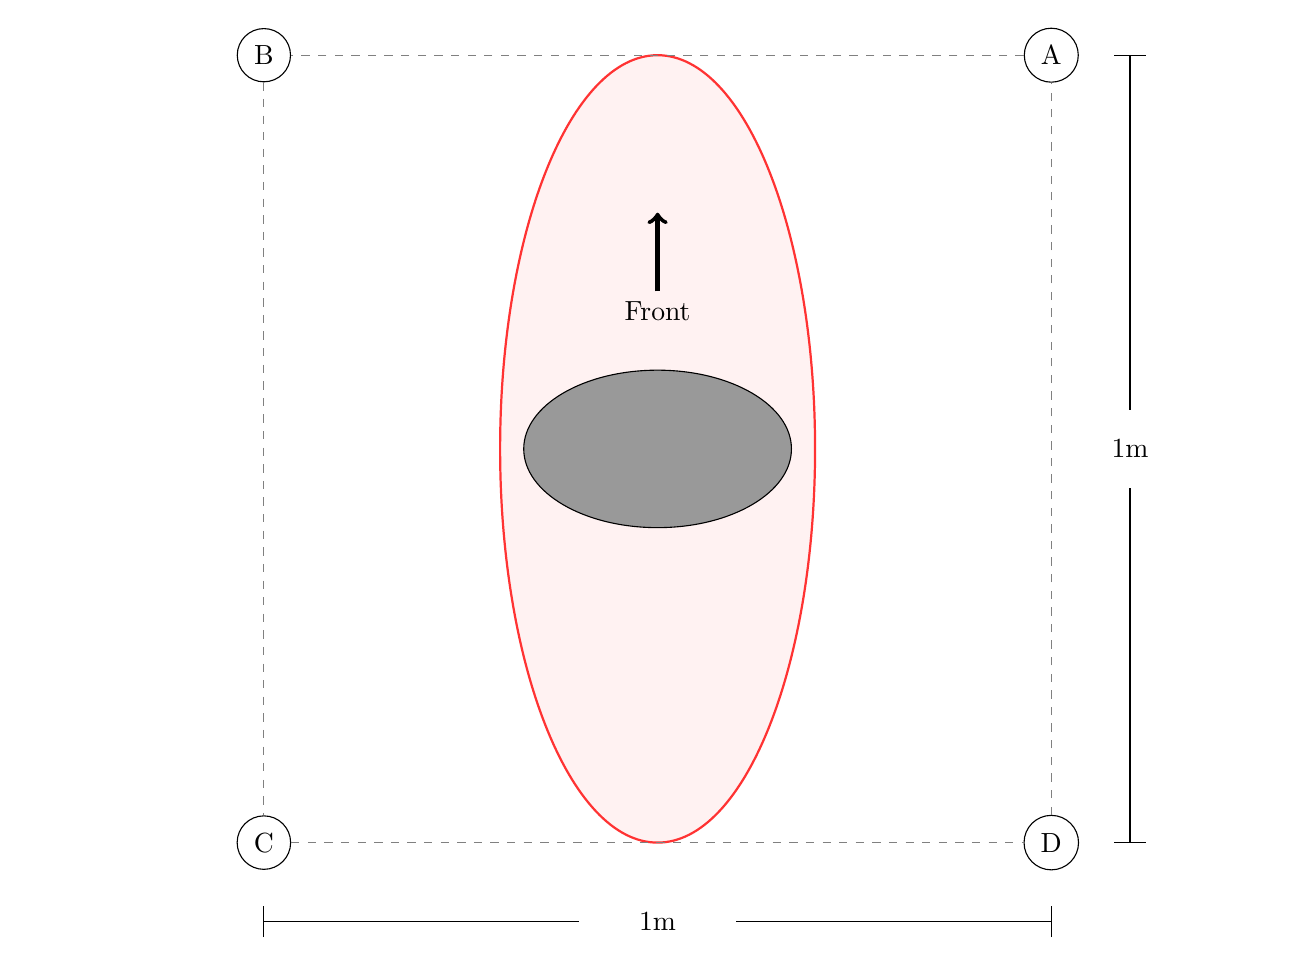
\begin{tikzpicture}[node distance=2cm]

\draw[help lines] (-5,-5) (5,5);

\node[hydrophone] (A) at (5,5)   {A};
\node[hydrophone] (B) at (-5,5)  {B};
\node[hydrophone] (C) at (-5,-5) {C};
\node[hydrophone] (D) at (5,-5)  {D};

% Draw the kayak
\draw[color=red!80,fill=red!5, thick] (0,0) ellipse (2 and 5);
\draw[fill=black!40] (0,0) ellipse (1.7 and 1);
\draw[->,ultra thick] (0,2) -- (0,3);
\node[below] at (0,2) {Front};

% Draw lines to hydrophones
\draw[color=gray,dashed]
	(A) -- (B)
	(B) -- (C)
	(C) -- (D)
	(D) -- (A)	
;

% Draw the measurements
\draw[]
	(6,0.5)  -- (6,5)    % vertial line
	(6,-0.5) -- (6,-5)   % vertial line
	(5.8,5)  -- (6.2,5)  % horizontal tick
	(5.8,-5) -- (6.2,-5) % horizontal tick
	
	(-5,-6)   -- (-1,-6)    % horizontal line
	(1,-6)    -- (5,-6)     % horizontal line
	(-5,-6.2) -- (-5,-5.8)  % vertical tick
	(5,-6.2)  -- (5,-5.8)   % vertical tick
;
\node[] at (6,0)  {1m};
\node[] at (0,-6) {1m};

% to center image (offsets measurement line on right)
\path[fill=none] (-8,0) (8,0);

\end{tikzpicture}
\end{center}
\caption{The hydrophone array attached to the kayak.}
\label{fig:array}
\end{figure}


%%%%%%%%%%%%%%%%%%%%%%%%%%%%%%%%%%%%%%%%%%%%%%%%%%%%%%%%%%%%%%%%%%%%%%%%%%%%%%%
\section{Software Setup}

\subsection{Loading Software}

It may at some point be necessary to add or replace code on one of the devices,
such as when new hardware is acquired or the software is updated.
To do this, the first step is to download (``clone'') the most recent copy
of the \texttt{master} branch from the
\href{https://github.com/cabeese/crab-tracker/}
{Crab Tracker GitHub repository}.
It is possible to download a ZIP file containing the contents of the repository
from the GitHub website.
Another option, however, is to use the \texttt{git} command-line utility to
make a clone.
To see if you have Git installed, open a shell/terminal and type \texttt{git}.
A usage page should be displayed.
If not, look online for instructions on how to install Git on your operating
system.

The steps shown in the remainder of this section are meant to be run on a
UNIX-like operating system (such as Linux, MacOS, or BSD).
However, equivalent commands exist for other systems, such as Windows.

\subsubsection{Downloading the source code}\label{sec:git}

The following instructions apply to both personal computers (which may be
used to upload code to the Arduino), and to the Raspberry Pi that is to be used
in the  field.

\textbf{If you have not cloned the repository} on this computer before, run:

\begin{lstlisting}[language=bash]
$ git clone https://github.com/cabeese/crab-tracker.git
$ cd crab-tracker
\end{lstlisting}

\textbf{If you have already cloned the repository} at some point previously,
\texttt{cd} into the project's directory and run \texttt{git pull}.

\subsubsection{Flashing code to the Arduino}

In order to upload binaries to the Arduino, you will need the Arduino software
from \href{https://www.arduino.cc/en/Main/Software}{their website}.

With the software downloaded, plug the Arduino into your computer.

Next, open the
\texttt{src/arduino-src/arduino-src.ino} file in the Arduino
editor.
Under the Tools menu, set the \textsl{Board} to \textit{Arduino Nano}
and set the \textsl{Port} to the port you plugged the Nano in to.

Now click the \textsc{Upload} button.
The compile and upload process should finish in a few seconds.

That's it!

\subsubsection{Updating code on the Pi}

To update the source code on the Raspberry Pi, connect the Pi to a power source
and to your network (e.g. via an Ethernet cable).
Attaching an external keyboard is highly recommended as well, though it is
possible
to use the on-screen keyboard if you do not have access to a physical one.

With the Pi connected, open up the Terminal app and use the commands listed
in Section \ref{sec:git} to download a copy of the source code.

Next, run the following commands to make the executable file.

\begin{lstlisting}[language=bash]
$ cd crab-tracker
$ cd src/pi-src
$ make
\end{lstlisting}

The output of the \texttt{g++} commands will be shown.
When the shell prompt reappears, you can start the program like so:

\begin{lstlisting}[language=bash]
$ ./crab-tracker
\end{lstlisting}

\subsection{Configuring Settings}

The main program on the Raspberry Pi has a few configuration options that can
be loaded at runtime (i.e. when the program starts up, as opposed to when the
source code is compiled into an executable file).
The configuration options are located in the \texttt{/etc/crab-tracker.conf}
file.
Use your favorite text editor to make changes to this file as needed.
The format for this file is simply a set of line-delimited key/value pairs,
where each key is an alphanumeric string and each value is an integer.
A single space character separates the key and value.
Lines beginning with a hash (\texttt{\#}) character are comments and will be
ignored by the program.
A sample version of the configuration file is located at
\href
{https://github.com/cabeese/crab-tracker/blob/master/src/crab-tracker.conf.example}
{\texttt{src/crab-tracker.conf.example}}.
An updated list of possible configuration parameters can be found in the
\href
{https://github.com/cabeese/crab-tracker/blob/master/src/pi-src/README.md}
{\texttt{src/pi-src/README.md}} file.

\subsection{Configuring a new Raspberry Pi}

If starting with a brand-new Raspberry Pi or simply a new Micro-SD Card,
follow the instructions found in
\href{https://github.com/cabeese/crab-tracker/blob/master/doc/model-B-config.md}
{doc/model-B-config.md}.

\end{document}

